
\documentclass[12pt,italian,a4paper,oneside,openright]{book}
\usepackage[a4paper,top=0 cm,bottom=4.5 cm,left=3 cm,right=3 cm]{geometry}
\usepackage{url,amsfonts,epsfig}
\usepackage[italian]{babel}
\usepackage[utf8]{inputenc}
\usepackage{lmodern}
%\usepackage[format=hang,font=footnotesize]{caption}
\usepackage{vmargin}
\usepackage{amsmath}
\usepackage{indentfirst}
\usepackage{listings}
\usepackage{graphicx}

\lstset{ %
  backgroundcolor=\color{white},   % choose the background color
  basicstyle=\footnotesize,        % size of fonts used for the code
  breaklines=true,                 % automatic line breaking only at whitespace
  captionpos=b,                    % sets the caption-position to bottom
  commentstyle=\color[rgb]{0,0.6,0},    % comment style
  escapeinside={\%*}{*)},          % if you want to add LaTeX within your code
  keywordstyle=\color{blue},       % keyword style
  stringstyle=\color[rgb]{0.58,0,0.82},     % string literal style
}



%\usepackage{algorithm,algorithmic}
\graphicspath{{img/}}
\usepackage[hyperindex]{hyperref} %per l'indice interattivo
\hypersetup{colorlinks=true, linkcolor=black} %per colorare i link
%\DeclareGraphicsRule{.jpg}{jpg}{}{} %da commentare per il PDF
%\DeclareGraphicsRule{.bmp} {bmp}{}{} %da commentare per il PDF
\setmarginsrb{35mm}{30mm}{30mm}{30mm}{0mm}{10mm}{0mm}{10mm}
%%\setmarginsrb{1.5cm}{1.5cm}{1,2cm}{1,5cm}{0cm}{2cm}{2cm}{2cm}

\title{Progetto di Riconoscimento e Classificazione di Forme}
\author{Marco Saviano}
%\date{14/12/2011}


\begin{document}

\pagenumbering{Roman}

%%%% Opzione per interlinea 2
\baselineskip 1.5em

%% FRONTESPIZIO
{ \thispagestyle{empty}


\vskip 1cm \large \centerline{\textsc{Universita' degli Studi di Napoli ``Parthenope''}}

\centerline {\textsc{Facolta' di Scienze e Tecnologie}}

\centerline {\small\textsc{Corso di laurea in Informatica Applicata}}

\begin{center}

\includegraphics[scale=0.24]{logo_parthenope}
\end{center}

\vskip 0.5cm

\large \centerline {\textsc{Progetto di Riconoscimento e Classificazione di Forme}}

\vskip 0.5cm

\Large \centerline {Deep Poselets for Human Detection}


\vskip 4.5cm


\large
\begin{minipage}[t]{7cm}
\textsc{Docente}

Alfredo Petrosino

\end{minipage}
\hfill
\begin{minipage}[t]{5cm}
\hfill \textsc{Candidato}

\hfill Marco Saviano
\hfill 0120000114\\
\end{minipage}

\vskip 2.0 cm \Large \centerline {Anno Accademico 2013-2014}
\vfill \eject}

% fine frontespizio

%%% DEDICA
%\thispagestyle{plain} \vspace*{\fill}
%\begin{flushright}
%\textit{``I computer sono incredibilmente veloci, accurati e stupidi.\\
%Gli uomini sono incredibilmente lenti, inaccurati e intelligenti.\\
%L'insieme delle due costituisce una forza incalcolabile.''}\\
%\emph{Albert Einstein} \vfill
%\end{flushright}

%\newpage
%\thispagestyle{plain}
\markboth{Indice}{Indice}
\tableofcontents
%%\listoffigures
%%\listoftables
\newpage

\pagenumbering{arabic}
\chapter*{Abstract} \label{abstract}
L'approccio sviluppato si rivolge al problema del rilevamento di persone in scene naturali utilizzando un metodo basato sul rilevamento di singole parti del corpo, chiamate poselet. Come prima fase si introduce un metodo per la raccolta di milioni di immagini etichettate per ogni tipo di poselet. Queste ultime vengono utilizzate per addestrare una Rete Neurale Convolutiva (CNN) per discriminare i vari tipi di poselet e separarle dallo sfondo. La CNN viene poi utilizzata per ottenere un vettore di caratteristiche per la poselet di 256 dimensioni. Si collezionano delle immagini per ogni tipo di poselet e si addestra un SVM per ciascun tipo di poselet utilizzando il vettore di caratteristiche precedentemente ottenuto. I classificatori SVM vengono utilizzati su patch dell'immagine target per individuare la presenza delle poselets che successivamente vengono combinate per trovare la posizione della persona intera.  
\chapter*{Introduzione} \label{cap0}
Il rilevamento di persone in scene naturali è molto impegnativo per problemi dovuti alla grande variabilità in apparenza, posa e occlusioni. Negli ultimi anni, anche grazie agli enormi passi avanti fatti in campo tecnologico, in letteratura sono sempre più presenti approcci basati sull'utilizzo delle Reti Neurali Convolutive (CNN). \\
L'approccio leader nelle performance in ImageNet e PASCAL è il R-CNN di Girschik \textit{et al.}\cite{rcnn}, il quale mostra come la localizzazione di persone (e altri oggetti) può essere effettuata dapprima individuando alcune possibili locazioni di persone o oggetti nell'immagine le quali vengono presentate successivamente ad una CNN che effettua la classificazione.\\
Uno dei problemi maggiori nell'utilizzo delle CNN per il rilevamento di persone è che la dimensione dell'input della CNN deve essere fissa mentre in realtà la parte di immagine può avere una proporzione arbitraria.\\
Nell'approccio di Girschik dall'immagine intera vengono estrapolate delle regioni con un metodo bottom-up le quali avranno differenti proporzioni: per adattare la dimensione della regione con la dimensione di input della CNN viene effettuata un'operazione di ridimensionamento, la quale può portare ad immagini molto distorte. Per ovviare a ciò oltre a campioni di addestramento con proporzioni originali vengono utilizzati nella fase di addestramento anche campioni distorti che non esistono in natura, i quali rendono più complesso al sistema l'apprendimento di corrispondenze di uno stesso oggetto. Un ulteriore limite della R-CNN è il metodo utilizzato nella fase preliminare di segmentazione dell'immagine in regioni dal quale dipende la bontà della classificazione finale.\\
Nel seguente lavoro viene proposto un nuovo approccio per il rilevamento di persone in immagini, il quale non prevede nella fase di addestramento l'utilizzo di campioni distorti in proporzioni e una grande variabilità di campioni per lo stesso classificatore. L'approccio utilizza le \textit{Poselets} presentate da Bourdev \textit{et al.}\cite{poselets}: esse sono parti del corpo umano in una particolare posa viste da uno specifico punto di vista. \\
Viene presentato un approccio deep learning che utilizza una CNN come estrattore delle caratteristiche delle poselets che produce un vettore di caratteristiche di sole 256 dimensioni.\\
Il resto dell'elaborato è diviso nel seguente modo. Nel capitolo 1 viene mostrata la struttura della Deep Net e la creazione del training-set, nel capitolo 2 vediamo come funzionano i classificatori Poselet, nel capitolo 3 ci sono dettagli sull'implementazione ed infine nell'ultimo capitolo vengono mostrati vari test.




\chapter{Deep Net} \label{cap1}
In questo capitolo si mostra come è stato creato il dataset per l'addestramento della Deep Net e la sua struttura.
\section{Training Set}
Nel primo lavoro, Bourdev come campioni di addestramento per ogni tipo di poselet ha utilizzato un dataset chiamato \textit{H3D} presentato nella medesima pubblicazione. In questo dataset vengono etichettate alcune zone particolari del corpo umano (naso, occhio destro/sinistro, orecchie, spalle etc.) come \textit{keypoints}. Una poselet è una regione dell'immagine dove sono presenti keypoints con una specifica configurazione spaziale. Quindi ad esempio possiamo avere una poselet relativa alla faccia vista in posizione frontale, oppure una poselet relativa alla parte superiore del corpo sempre vista in posizione frontale

\begin{figure}[h!b]
 \centering
 \subfloat {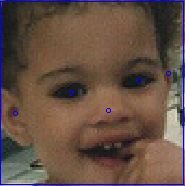
\includegraphics[width=4cm]{cap1/poselet1.jpg}}
 \hspace{5mm}
 \subfloat {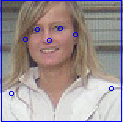
\includegraphics[width=4cm]{cap1/poselet2}}
 \caption{A sinistra poselet con 5 keypoints, a destra 7 keypoints}
 \end{figure}
 
 Nel primo lavoro basato su HOG, per ogni tipo di poselet (sono stati estratti 150 tipi di poselets\cite{poselets-image}) vengono raccolti i campioni utilizzando le immagini presenti nel dataset H3D.\\
 In questo approccio utilizziamo una CNN come estrattore di caratteristiche.
 
 \begin{figure}[h!b]
 \centering
 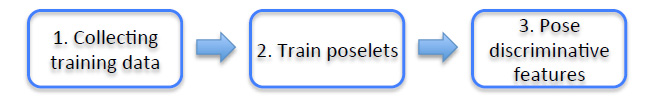
\includegraphics[scale=0.5]{cap1/train}
 \caption{Fasi di addestramento della Deep Net}
 \label{}
 \end{figure}
 
 
 
 Uno dei problemi maggiori che affligge l'utilizzo delle CNN è che necessitano di un numero enorme di campioni di addestramento per evitare il fenomeno dell'overfitting. Le immagini presenti nel dataset H3D non bastano e quindi viene presentato un approccio per ottenere il numero necessario di campioni.\\
 E' stato utilizzato il software pubblicamente disponibile\cite{poselet-code} relativo al primo lavoro di Bourdev sulle poselets utilzzando HOG come estrattore di caratteristiche. Come dataset è stato utilizzato COCO\cite{coco} il quale contiene circa 50000 immagini di persone con relative ground truth. Sono stati estratti i bounding boxes individuati dal software: ciascun bounding box è supportato da un insieme di attivazioni-poselet le quali sono etichettate positive se il bounding box relativo e la ground truth danno un intersection-over-union di almeno 0.5, altrimenti negative.
 
\begin{figure}[h!b]
\centering
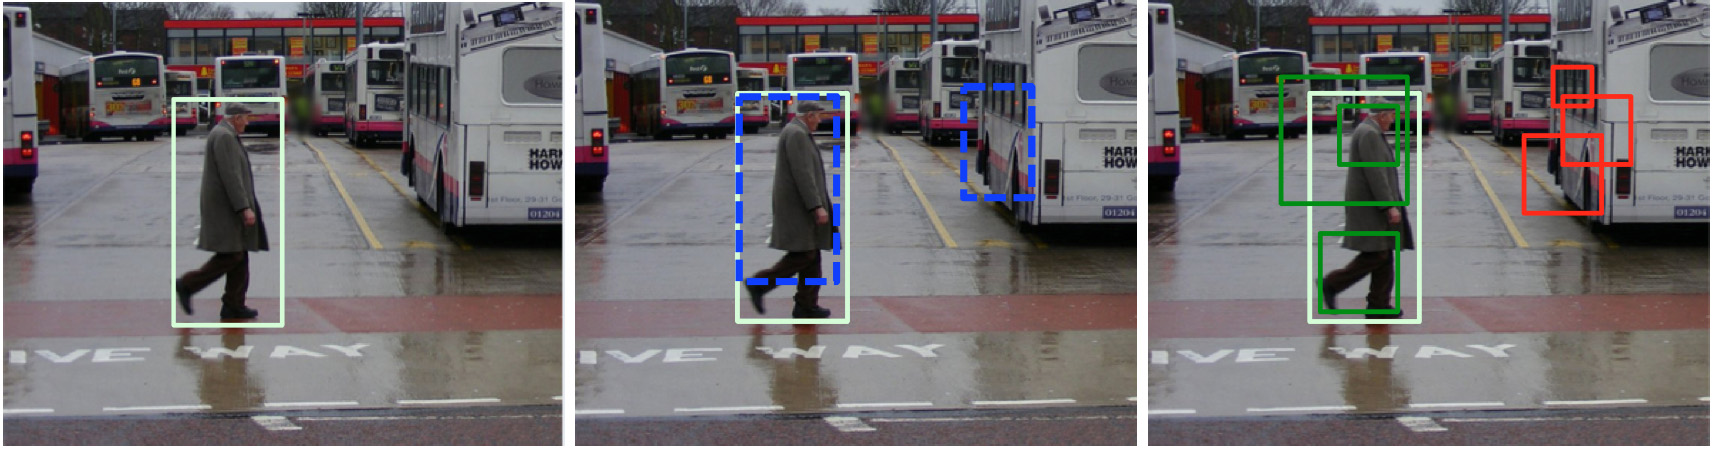
\includegraphics[scale=0.25]{cap1/act_label}
\caption{\textbf{Sinistra:} persona con relativa ground truth \textbf{Centro:} in blu bounding boxes rilevati \textbf{Destra:} in verde attivazioni positive, in rosso negative }
\label{}
\end{figure}

Il metodo illustrato permette di ottenere circa 20000 immagini per ciascun tipo di poselet, per un totale di 3 milioni di campioni positivi. Si ottengono inoltre circa 2 milioni di immagini di background.

\section{Deep Net}
Nella tabella \ref{table-deepnet} viene mostrata la struttura della Deep Net. L'input è una patch RGB di dimensioni 61x61x3 estratta tramite ridimensionamento dalle attivazioni-poselet: ad esse è stata sottratta la media. 

\begin{table}[h!b]
\centering
\begin{tabular}{|l | c | c | c | c | c | c|}
 \hline
 Layer & 1 & 2 & 3 & 4 & 5 & 6 \\ \hline
 Stage & conv+max & conv & conv & conv & full & full \\ \hline
 \#channels & 64 & 256 & 128 & 128 & 256 & 5 \\ \hline
 Filter Size & 5x5 & 5x5 & 3x3 & 3x3 & - & - \\ \hline
 Conv Stride & 2x2 & 1x1 & 1x1 & 1x1 & - & - \\ \hline
 Pooling Size 3x3 & - & -& -& -& - & -\\ \hline
 Pooling Stride 2x2 & - & -& -& -& - & - \\ \hline
 Zero Padding Size - & - & -& -& -& - & - \\ \hline 
 Spacial input size & 61x61x3 & 14x14 & 10x10 & 8x8 & 6x6 & 1x1 \\
 \hline
\end{tabular}
\caption{Struttura Deep Net}
\label{table-deepnet}
\end{table}

Visto l'enorme onere computazionale, in questa implementazione al posto di classificare una patch tra 151 classi (150 tipi di poselet più background) si è scelto di utilizzare un numero di classi pari a 5 (4 tipi di poselets e background). Quindi la prima classe corrisponde al tipo poselet 16, la seconda classe il tipo 144, la terza il tipo 97 e la quarta il tipo 86. Ricordiamo che è possibile vedere i vari tipi di poselets al seguente link\cite{poselets-image}.

\begin{figure}[h!b]
 \centering
 \subfloat {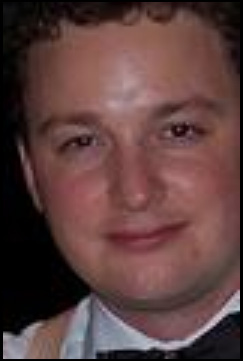
\includegraphics[width=3cm]{cap1/pos11}}
 \hspace{3mm}
 \subfloat {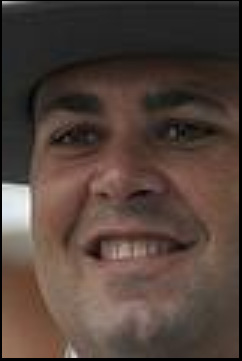
\includegraphics[width=3cm]{cap1/pos12}}
 \hspace{3mm}
 \subfloat {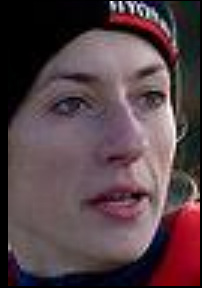
\includegraphics[width=3cm]{cap1/pos13}}
 \hspace{3mm}
 \subfloat {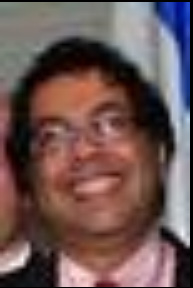
\includegraphics[width=3cm]{cap1/pos14}}
 \caption{Esempi di immagini della prima classe (\#poselet 16)}
 \end{figure}
 
 \begin{figure}[h!b]
 \centering
 \subfloat {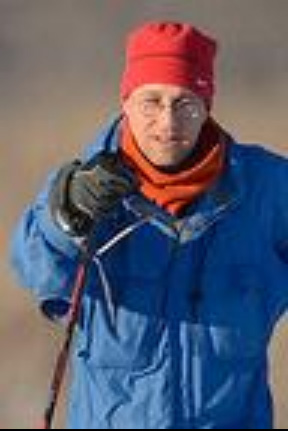
\includegraphics[width=3cm]{cap1/pos21}}
 \hspace{3mm}
 \subfloat {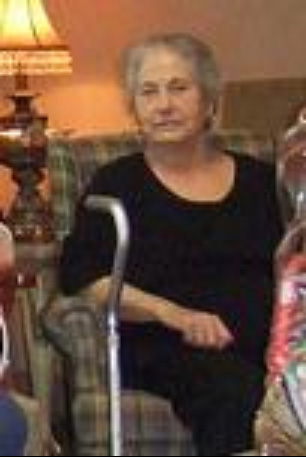
\includegraphics[width=3cm]{cap1/pos22}}
 \hspace{3mm}
 \subfloat {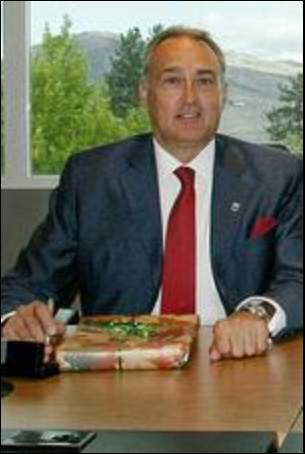
\includegraphics[width=3cm]{cap1/pos23}}
 \hspace{3mm}
 \subfloat {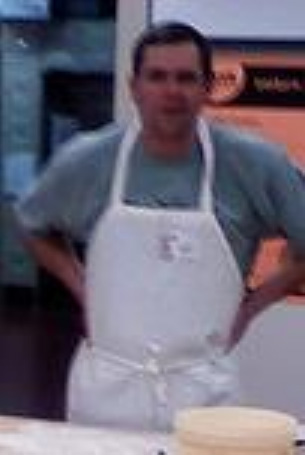
\includegraphics[width=3cm]{cap1/pos24}}
 \caption{Esempi di immagini della seconda classe (\#poselet 144)}
 \end{figure}
 
  \begin{figure}[h!b]
 \centering
 \subfloat {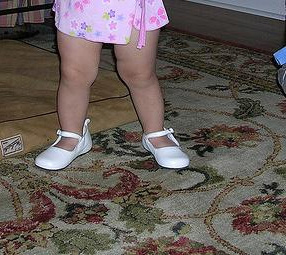
\includegraphics[width=3cm]{cap1/pos31}}
 \hspace{3mm}
 \subfloat {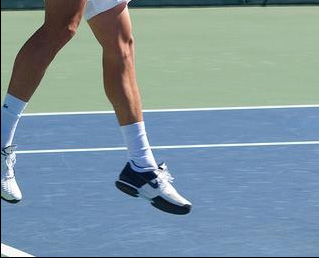
\includegraphics[width=3cm]{cap1/pos32}}
 \hspace{3mm}
 \subfloat {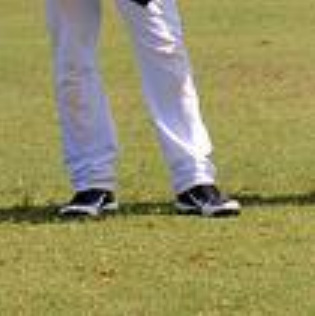
\includegraphics[width=3cm]{cap1/pos33}}
 \hspace{3mm}
 \subfloat {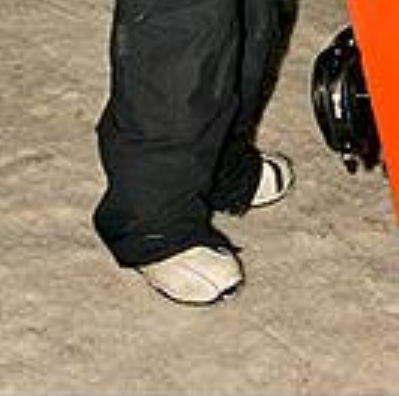
\includegraphics[width=3cm]{cap1/pos34}}
 \caption{Esempi di immagini della terza classe (\#poselet 97)}
 \end{figure}
 
 \begin{figure}[h!b]
 \centering
 \subfloat {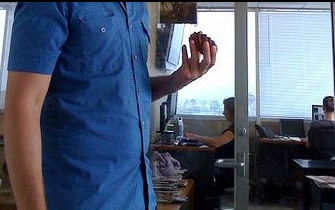
\includegraphics[width=3cm]{cap1/pos41}}
 \hspace{3mm}
 \subfloat {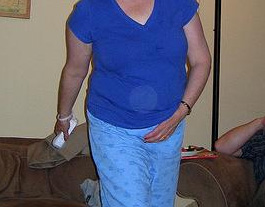
\includegraphics[width=3cm]{cap1/pos42}}
 \hspace{3mm}
 \subfloat {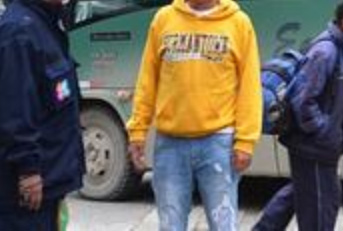
\includegraphics[width=3cm]{cap1/pos43}}
 \hspace{3mm}
 \subfloat {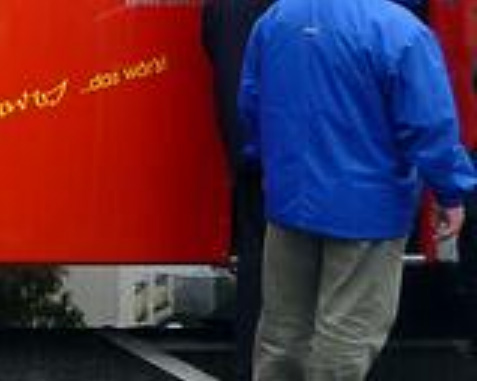
\includegraphics[width=3cm]{cap1/pos44}}
 \caption{Esempi di immagini della quarta classe (\#poselet 86)}
 \end{figure}
 
 Le immagini sono state divise in 72 batch, ognuno contenente 250 campioni positivi per ogni classe e 700 negativi: in totale sono state processate 122400 immagini campione. Il learning rate iniziale è stato impostato a 0.15, utilizzando il valore 1e-5 per il weigth-decay e 0.9 per il momentum.


\begin{figure}[h!b]
\centering
  
  \[\Delta w_i(t+1)=w_i-n\frac{\delta E}{\delta w_i}+\alpha \Delta w_i(t) -\lambda \eta w_i \]
  \caption{Aggiornamento Parametri. ${\alpha}$  momentum. ${\lambda}$ weight-decay. ${\eta}$ learning-rate}
\end{figure}
 
L'utilizzo del weight-decay penalizza i grossi cambiamenti di parametri tra un passo e l'altro, mentre il momentum permette di diminuire le fluttuazioni dei cambiamenti di parametri tra un iterazione e l'altra. Si è riusciti ad ottenere un errore di classificazione di circa il 9\% su un validation-set composto da 600 campioni: 150 campioni positivi per ogni classe e 150 campioni negativi.
 
 
 
 
\chapter{Classificatori Poselets} \label{cap2}
In questo capitolo viene presentato il procedimento per ottenere i classificatori relativi ai 4 tipi di poselets presi in considerazione. Successivamente vediamo come vengono raggruppate le attivazioni-poselet per ottenere il bounding box della persona.

\section{Addestramento Classificatore Poselet}
Il procedimento per l'addestramento dei Classificatori Poselet è raffigurato in \ref{class-pos}

\begin{figure}[h]
\centering
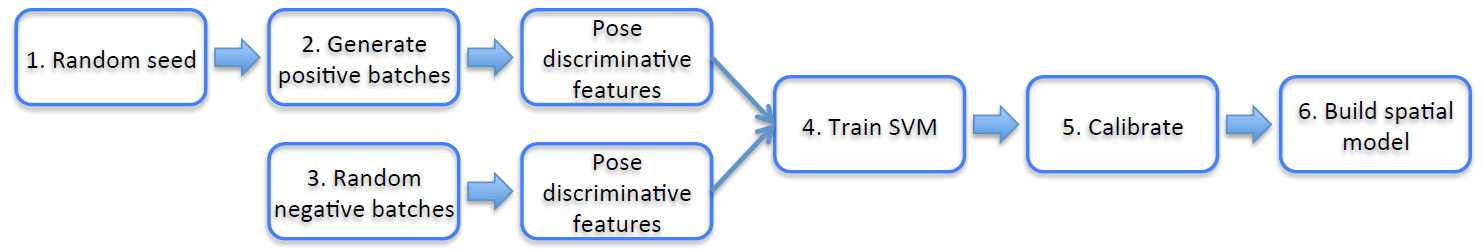
\includegraphics[scale=0.28]{cap2/class-pos}
\caption{Fasi addestramento classificatore poselet}
\label{class-pos}
\end{figure}

\subsection{Random Seed}
Il primo passo è quello di ottenere il \textit{Random Seed}: essa è una patch contenente un gruppo di keypoints in una particolare configurazione spaziale (faccia, due gambe, busto etc.) . Partendo dal Seed, cerchiamo nel training-set altre regioni che hanno la stessa configurazione spaziale dei keypoints. In questo caso è stato utilizzato come dataset PASCAL 2011\cite{pascal2011}, grazie alle annotazioni dei keypoints rilasciate su di esso\cite{pascal-keypoints}.\\

\subsection{Generazione campioni positivi}
Per trovare due regioni con la stessa configurazione di keypoints, utilizziamo la seguente distanza nello spazio 3D:

\begin{figure}[h]
\centering
  $d_s(r)=\sum_{i}w_s(i)||x_s(i)-x_r(i)||_2^2(1+h_{s,r}(i))$
  \caption{Distanza tra la configurazione di keypoint \textit{s} e \textit{r}}
\end{figure}

dove x$_s$(i)=[x,y,z] sono le coordinate 3D normalizzate dell'i-esimo keypoint di s. Il termine $w_s(i)\propto exp(-x_s(i)^2/(2\sigma ^2))$ è la Gaussiana con media nel centro della patch. $h_s,r(i)$ è una penalità basata sulla mancata corrispondenza di visibilità del keypoint \textit{i} nelle due regioni. Se il keypoint \textit{i} è visibile o invisibile in entrambe le regioni allora $h_s,r(i)=0$, altrimenti $h_s,r(i)=a, a>0$. Possiamo inoltre avere che il \textit{i}-th keypoint è presente in una regione ed assente in un altra: in questo caso il termine rispettivo è $w_s(i)b$ dove $(\sigma,\alpha,b,h)$ sono parametri fissati del modello.\\

\begin{figure}[h]
\centering
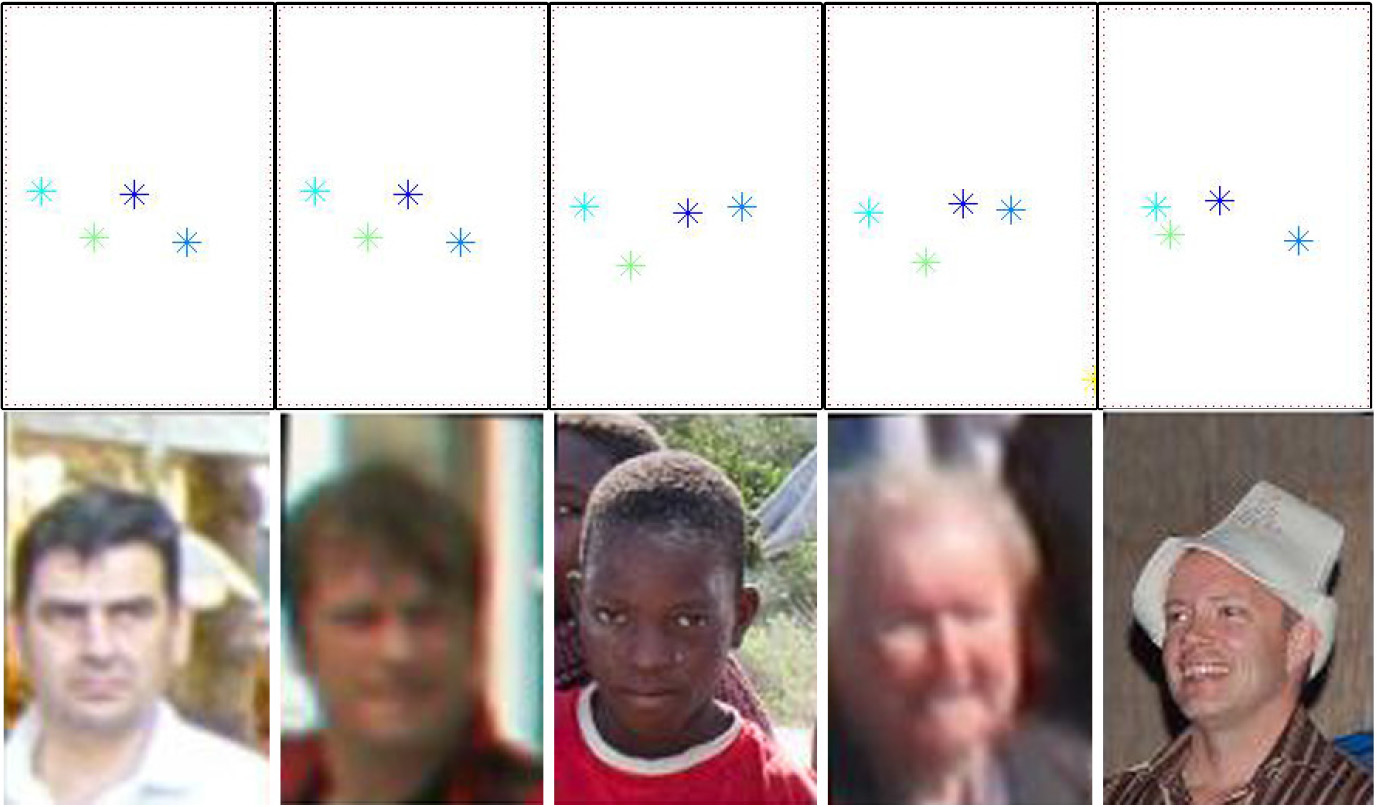
\includegraphics[scale=0.28]{cap2/face-keys}
\caption{Regioni con distribuzione dei keypoints simile}
\label{}
\end{figure}

\begin{figure}[h]
\centering
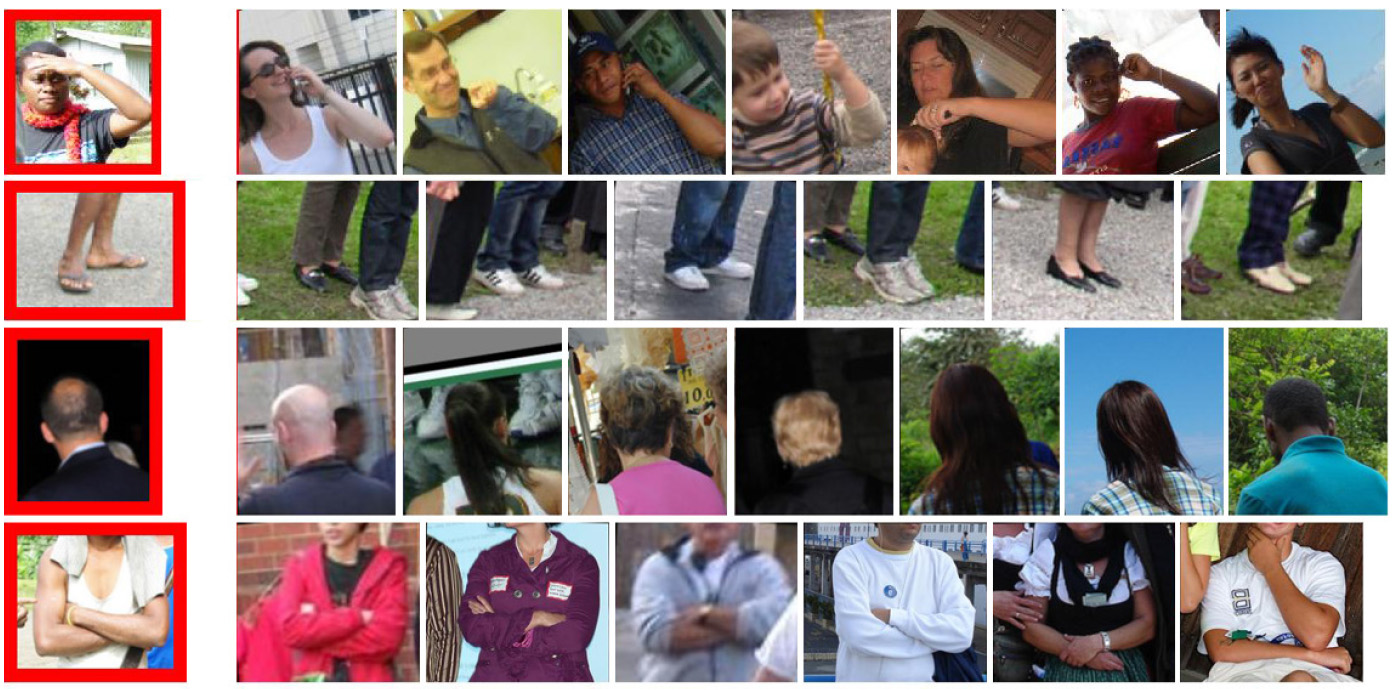
\includegraphics[scale=0.28]{cap2/pos-matches}
\caption{Sulla sinistra troviamo le regioni di query e i risultati ottenuti}
\label{}
\end{figure}

\subsection{Estrazione Caratteristiche}
Per estrarre le caratteristiche di ogni singola regione utilizziamo la Deep Net precedentemente addestrata. Eliminiamo dalla struttura l'ultimo layer (softmax layer) e utilizziamo il vettore di 256 dimensioni come vettore delle caratteristiche.

\subsection{Addestramento Classificatore}
Una volta scelto il Random Seed, collezionato regioni con configurazione di keypoints simile (campioni positivi) e scelto a caso campioni negativi, estraiamo per ogni regione il vettore delle caratteristiche e utilizziamo questi per addestrare un semplice classificatore SVM. Dopo aver addestrato per la prima volta l'SVM, applichiamo il classificatore ad una serie di regioni di immagini che non presentano persone all'interno. Prendiamo le regioni classificate come positive (sono dei falsi positivi), le aggiungiamo ai campioni negativi precedentemente collezionati e addestriamo nuovamente un SVM: questo procedimento permette di diminuire il tasso di rilevamento di falsi positivi.\\
Una volta addestrato il classificatore, eseguiamo la classificazione sui campioni positivi: l'SVM darà per ognuno di essi uno score. Per limitare il firing-rate di ciascun classificatore, selezioniamo il k-simo score e lo imponiamo come limite inferiore per il quale un campione viene classificato come positivo.\\
Dopo aver calibrato il firing-rate, diamo ad ogni classificatore uno score in dipendenza della sua bontà. Per fare ciò applichiamo il classificatore alle immagini che contengono le poselet-patch utilizzate per addestrare l'SVM ed etichettiamo le attivazioni-poselet individuate: essa sarà etichettata come positiva se l'intersection-over-union è almeno di 0.5 con la poselet patch presente nell'immagine. Una volta etichettate tutte le attivazioni-poselet e avendo i relativi score SVM, addestriamo un regressore logistico per convertire gli score in probabilità.

\begin{figure}[h]
 \centering
 \subfloat {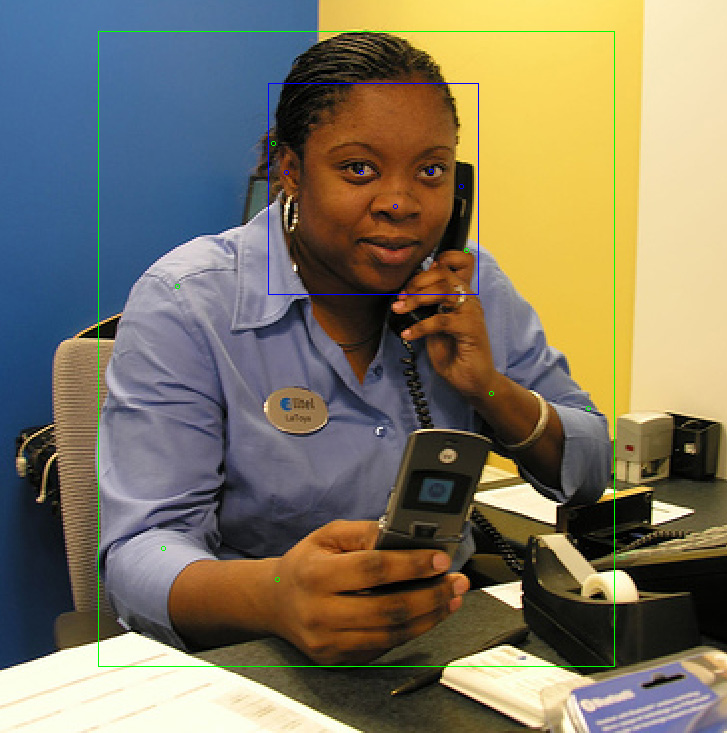
\includegraphics[scale=0.28]{cap2/image-patch}}
 \newline
 \subfloat {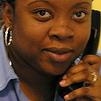
\includegraphics[scale=0.7]{cap2/act-pos1}}
 \hspace{5mm}
 \subfloat {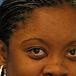
\includegraphics[scale=0.7]{cap2/act-pos2}}
 \hspace{5mm}
 \subfloat {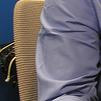
\includegraphics[scale=0.7]{cap2/act-neg}}
 \caption{In \textbf{alto} immagine del training set con relativa poselet-patch (in blu) e keypoints. In \textbf{basso} le prime due attivazioni-poselet sono etichettate come positive mentre la terza negativa}
 \end{figure}

A questo punto scegliamo un gruppo di classificatori poselet i quali avranno una buona probabilità di successo e si differenziano sulle zone del corpo da rilevare.\\

\subsubsection{Stima distribuzione keypoints e bounding boxes}
Nell'ultima fase di addestramento viene creato un modello spaziale: per ogni classificatore viene eseguita la stima della distribuzione dei keypoints e la predizione del bounding box.\\
Per la predizione dei keypoints eseguiamo il seguente procedimento: per ogni immagine utilizzata nella fase di addestramento dell'SVM, poniamo il centro del sistema di riferimento al centro della poselet-patch e calcoliamo la gaussiana relativa alla distribuzione dello spazio di ciascun keypoint: questo viene fatto per tutti i 20 keypoints anche se essi sono presenti fuori la poselet-patch o non presenti in qualche immagine. In questo modo avremo che se per esempio consideriamo la poselet-patch relativa alla faccia, avremo distribuzioni "piccate" in corrispondenza degli occhi e del naso.\\ \\
Per quanto riguarda la predizione del bounding box, portiamo sempre il centro del sistema di riferimento nel centro della poselet-patch e calcoliamo la media dei bounding boxes di tutte le immagini: il bounding box è definito dalle coordinate 2D dell'angolo alto-sinistro e basso-destro. In questo modo avremo che se consideriamo il bounding box predetto da un classificatore relativo alla poselet faccia, avremo che il lato superiore del bounding box sarà vicino al lato superiore della poselet-patch, mentre il lato inferiore sarà più distante (distanza piedi faccia): ovviamente se consideriamo il classificatore relativo alla poselet gambe è l'inverso.

\section{Funzionamento Classificatori}
In figura \ref{class-test} viene mostrato il procedimento per l'individuazione dei bounding box delle persone in immagini utilizzando i classificatori precedentemente addestrati.

\begin{figure}[h]
\centering
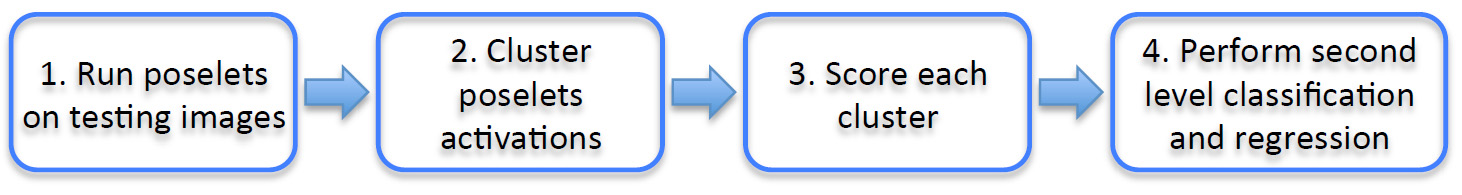
\includegraphics[scale=0.28]{cap2/class-test}
\caption{Rilevamento bounding boxes}
\label{class-test}
\end{figure}

Vengono estratte delle regioni dell'immagine di test tramite una finestra di dimensioni fissa 61x61 (dimensione input CNN) che si muove sull'intera immagine a varie scale: le regioni estratte dall'immagine scalata (scale diverso da 1) vengono ridimensionate a 61x61. Queste regioni vengono classificate con gli SVM relativi ai vari classificatori poselet e quindi vengono raccolte una serie di attivazioni.\\
Una volta ottenute le attivazioni, esse vengono clusterizzate col seguente approccio: prese le distribuzioni dei keypoint del classificatore relativo all'attivazione, le posizioniamo nello spazio immagine e inseriamo nello stesso cluster due attivazioni le quali distribuzioni hanno una KL-Divergence simmetrica minore di una certa soglia. Essa viene calcolata per ogni keypoint e viene effettuata la somma: in questo modo si considerano le distribuzioni dei singoli keypoints indipendenti tra loro.

\begin{figure}[h]
\centering
  $\sum \frac{ \sigma_1 + \Delta \mu ^2}{\sigma_2} + \frac{\sigma_2 + \Delta \mu^2}{\sigma_1} $
  \caption{KL-Divergence simmetrica}
\end{figure}

Ogni cluster avrà un proprio score che è dato dalla somma degli score delle attivazioni al suo interno. Per ciascun cluster portiamo nello spazio immagine le varie predizioni dei bounding boxes per ciascuna attivazione: la predizione finale del bounding box relativo al cluster sarà la media dei bounding boxes di tutte le attivazioni, ognuno pesato col suo score.\\

Nell'ultima fase i bounding boxes ottenuti vengono immessi in un'altra CNN, la R-CNN\cite{r-cnn}: essa permette la classificazione di una regione in differenti categorie, tra cui la categoria persona. 






\chapter{Dettagli Implementativi} \label{cap3}
In questo capitolo sono presentati alcuni dettagli implementativi dell'approccio e vari test.

\section{Dettagli implementativi}
Per l'implementazione del software è stato utilizzato Matlab\cite{matlab}. L'implementazione della Deep Net è stata effettuata utilizzando il framework python Theano\cite{theano}: in esso sono state utilizzate le librerie di pylearn2\cite{pylearn2} per velocizzare l'operazione di convoluzione di tre volte\cite{conv-3x}. Anche se il software è stato implementato su sistema operativo Microsoft Windows 8.1, esso può funzionare anche su sistemi Unix come Mac OS e Linux a condizione che sia presente una GPU NVIDIA compatibile con CUDA\cite{cuda}, questo perché le librerie prelevate da pylearn2 funzionano solo tramite esso.\\
Il codice e i modelli pre-trained di R-CNN possono essere scaricati dal repository GitHub: esso utilizza come framework per la creazione della CNN Caffe\cite{caffe} il quale è provvisto di funzioni wrapper per l'utilizzo in Matlab.
Di seguito troviamo i dettagli del software utilizzato:

\begin{itemize}
\item Sistema Operativo Microsoft Windows 8.1
\item Matlab 2013a
\item Python 2.7.9
\item Theano 0.7.0 (importante utilizzare questa versione o superiore)
\item Caffe (scaricare l'ultima versione con le nuove funzioni wrapper Matlab)
\end{itemize}

Nella fase di addestramento dell'SVM, per ogni classificatore sono stati presi 700 campioni positivi (di cui 400 utilizzati come training-set) e 800 campioni negativi. I campioni sono stati presi tutti come regioni quadrate così da diminuire le distorsioni nell'operazione di ridimensionamento ad una patch di 61x61.\\

Nell'utilizzo dei classificatori per l'individuazione dei bounding boxes, l'immagine viene scalata agli scale 1.2, 1, 0.8, 0.6, 0.4 e 0.2.

\section{Implementazione Deep-Net}
Come detto precedentemente, la CNN è stata implementata utilizzando il framework python Theano. Di seguito vediamo la parte di codice per l'implementazione della struttura della CNN. 

\begin{lstlisting}[language=Python]
#Build the deep-net structure using Theano Framework
print "Building model..."
layer0_input = x.reshape((batch_size, 3, 61, 61))
# build symbolic expression that computes the convolution of input with filters in w
conv_out1=MyConvnetLayer(rng,input=layer0_input,filter_shape=(64, 3, 5, 5),image_shape=(batch_size, 3, 61, 61),conv_stride=(2,2),pool_stride=(2,2),poolsize=(3,3))

conv_out2=MyConvnetLayer(rng,input=conv_out1.output,filter_shape=(256,64,5,5),image_shape=(batch_size,64, 14, 14),conv_stride=(1,1))

conv_out3=MyConvnetLayer(rng,input=conv_out2.output,filter_shape=(128,256,3,3),image_shape=(batch_size, 256, 10, 10),conv_stride=(1,1))

conv_out4=MyConvnetLayer(rng,input=conv_out3.output,filter_shape=(128,128,3,3),image_shape=(batch_size, 128, 8, 8),conv_stride=(1,1))

layer5_input = conv_out4.output.flatten(2)

# construct a fully-connected sigmoidal layer
full_5 = HiddenLayer(
        rng,
        input=layer5_input,
        n_in=128 * 6 * 6,
        n_out=256,
        activation=T.tanh
)
# classify the values of the fully-connected sigmoidal layer
full_5_softmax = LogisticRegression(input=full_5.output, n_in=256, n_out=5)
weight_decay=1e-5
momentum=0.9

# Cost function for minibatch
cost = T.mean(T.nnet.categorical_crossentropy(full_5_softmax.p_y_given_x,y))
# Concatenation of the params
params=full_5_softmax.params + full_5.params + conv_out4.params + conv_out3.params + conv_out2.params + conv_out1.params
# create theano function to compute filtered images
train_model = theano.function([x,y,lr],
          [cost,full_5_softmax.p_y_given_x,full_5_softmax.y_pred,full_5_softmax.errors(y)],
          updates= gradient_updates_momentum(cost, params, lr, momentum,weight_decay),
          #updates=updates,
          allow_input_downcast=True,on_unused_input='ignore'
        )
\end{lstlisting} 

Qui viene riportata la function relativa all'aggiornamento dei parametri.

\begin{lstlisting}[language=Python]
#Weight update rule (using momentum and weightdecay)
def gradient_updates_momentum(cost, params, learning_rate, momentum,weight_decay):
    assert momentum < 1 and momentum >= 0
    # List of update steps for each parameter
    updates = []
    # Just gradient descent on cost
    for param in params:
        # For each parameter, we'll create a param_update shared variable.
        # This variable will keep track of the parameter's update step across iterations.
        # We initialize it to 0
        param_update = theano.shared(param.get_value()*0., broadcastable=param.broadcastable)
        # Each parameter is updated by taking a step in the direction of the gradient.
        # However, we also "mix in" the previous step according to the given momentum value.
        # Note that when updating param_update, we are using its old value and also the new gradient step.
        #updates.append((param, param - learning_rate*param_update))
        updates.append((param, param - learning_rate*param_update - param_update*weight_decay*learning_rate))
        # Note that we don't need to derive backpropagation to compute updates - just use T.grad!
        updates.append((param_update, momentum*param_update + (1. - momentum)*T.grad(cost, param)))
    return updates
\end{lstlisting}


\chapter{Test} \label{cap4}
In questo capitolo finale vengono presentati alcuni test effettuati nelle varie fasi dell'approccio precedentemente elencate. Come primo test vediamo la bontà dei vari classificatori-poselet. Successivamente vengono mostrati alcuni test di esecuzione.

\section{Classificatori Poselet}
Sono stati addestrati 7 tipi di classificatori-poselet: per ognuno di essi abbiamo da 1 a 3 classificatori: i classificatori di ogni tipo avranno gli stessi keypoints ma possono disporsi in modo differente nello spazio. Vediamo in dettaglio il loro numero e il tipo di poselet classificato

\begin{itemize}
\item 3 classificatori per la poselet contenente i keypoints: Occhio Sinistro/Destro, Naso, Orecchio Sinistro %face1
\item 2 classificatori per la poselet contenente i keypoints: Occhio Sinistro/Destro, Naso, Orecchio Sinistro/Destro %face12
\item 3 classificatori per la poselet contenente i keypoints: Occhio Sinistro/Destro, Naso, Orecchio Destro %face13
\item 3 classificatori per la poselet contenente i keypoints: Occhio Sinistro/Destro, Naso, Orecchio Sinistro/Destro, Spalla Sinistra/Destra, Gomito Sinistro/Destro %frontal2
\item 3 classificatori per la poselet contenente i keypoints: Occhio Sinistro/Destro, Naso, Orecchio Sinistro/Destro, Spalla Sinistra/Destra, Fianchi Sinistro/Destro %frontal22
\end{itemize}

Come è facilmente deducibile leggendo i keypoints presenti nei vari classificatori, essi individuano la parte superiore del corpo, soprattutto la zona relativa la faccia. Con questi classificatori quindi siamo abbastanza in grado di rilevare la parte superiore di persone poste in modo frontali a noi.\\
Per ogni classificatore poselet, riportiamo in basso la loro matrice di confusione e una poselet-patch presa dal training set: il classificatore è stato applicato a 300 campioni positivi e 800 campioni negativi. Tutti questi campioni non sono stati utilizzati nella fase di training. 

\begin{figure}[h]
 \centering
 \subfloat {\includegraphics[width=3cm]{cap4/ace1_11}} 
 \hspace{5mm}
 \subfloat {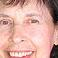
\includegraphics[width=3cm]{cap4/face1_2}}
 \hspace{5mm}
 \subfloat {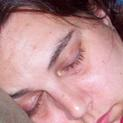
\includegraphics[width=3cm]{cap4/face1_3}}
 \vspace{5mm}
 
  \resizebox{.2\textwidth}{!}{%
 \begin{tabular}{|c | c|}
 \hline
 271 & 30 \\ \hline
 3 & 497 \\ 
 \hline
\end{tabular}%
}
\hspace{5mm}
\resizebox{.2\textwidth}{!}{%
\begin{tabular}[scale=1.5]{|c | c|}
 \hline
 265 & 36 \\ \hline
 14 & 486 \\ 
 \hline
\end{tabular}%
}
\hspace{5mm}
\resizebox{.2\textwidth}{!}{%
\begin{tabular}[scale=1.5]{|c | c|}
 \hline
 259 & 42 \\ \hline
 22 & 478 \\ 
 \hline
\end{tabular}%
}
\caption{Matrici di confusione per i classificatori-poselets tipo 1}
\label{table-deepnet}
 \end{figure}


\begin{figure}[h]
 \centering
 
 \subfloat {
\includegraphics[width=3cm]{cap4/face12_1}} 
 \hspace{5mm}
 \subfloat {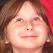
\includegraphics[width=3cm]{cap4/face12_2}}
 \vspace{5mm}
 
\resizebox{.2\textwidth}{!}{%
\begin{tabular}[scale=1.5]{|c | c|}
 \hline
 271 & 30 \\ \hline
 0 & 500\\ 
 \hline
\end{tabular}%
}
\hspace{5mm}
\resizebox{.2\textwidth}{!}{%
\begin{tabular}[scale=1.5]{|c | c|}
 \hline
 271 & 30 \\ \hline
 8 & 492 \\ 
 \hline
\end{tabular}%
}
\caption{Matrici di confusione per i classificator-poselets tipo 2}
\label{table-deepnet}
 \end{figure}



\begin{figure}[h]
 \centering
 \subfloat {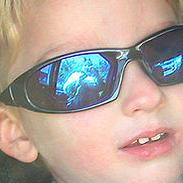
\includegraphics[width=3cm]{cap4/face13_1}} 
 \hspace{5mm}
 \subfloat {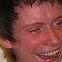
\includegraphics[width=3cm]{cap4/face13_2}}
 \hspace{5mm}
 \subfloat {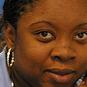
\includegraphics[width=3cm]{cap4/face13_3}}
 \vspace{5mm}
 
  \resizebox{.2\textwidth}{!}{%
 \begin{tabular}{|c | c|}
 \hline
 266 & 35 \\ \hline
 8 & 492 \\ 
 \hline
\end{tabular}%
}
\hspace{5mm}
\resizebox{.2\textwidth}{!}{%
\begin{tabular}[scale=1.5]{|c | c|}
 \hline
 253 & 48 \\ \hline
 31 & 469 \\ 
 \hline
\end{tabular}%
}
\hspace{5mm}
\resizebox{.2\textwidth}{!}{%
\begin{tabular}[scale=1.5]{|c | c|}
 \hline
 276 & 25 \\ \hline
 44 & 456 \\ 
 \hline
\end{tabular}%
}
\caption{Matrici di confusione per i classificatori-poselets tipo 3}
\label{table-deepnet}
 \end{figure}


\begin{figure}[h]
 \centering
 \subfloat {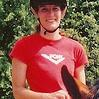
\includegraphics[width=3cm]{cap4/frontal2_1}} 
 \hspace{5mm}
 \subfloat {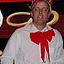
\includegraphics[width=3cm]{cap4/frontal2_2}}
 \hspace{5mm}
 \subfloat {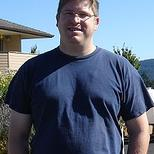
\includegraphics[width=3cm]{cap4/frontal2_3}}
 \vspace{5mm}
 
  \resizebox{.2\textwidth}{!}{%
 \begin{tabular}{|c | c|}
 \hline
 223 & 78 \\ \hline
 61 & 439 \\ 
 \hline
\end{tabular}%
}
\hspace{5mm}
\resizebox{.2\textwidth}{!}{%
\begin{tabular}[scale=1.5]{|c | c|}
 \hline
 22 & 279 \\ \hline
 0 & 500 \\ 
 \hline
\end{tabular}%
}
\hspace{5mm}
\resizebox{.2\textwidth}{!}{%
\begin{tabular}[scale=1.5]{|c | c|}
 \hline
 227 & 74 \\ \hline
 70 & 430 \\ 
 \hline
\end{tabular}%
}
\caption{Matrici di confusione per i classificatori-poselets tipo 4}
\label{table-deepnet}
 \end{figure}
 
 
 
 \begin{figure}[h!b]
 \centering
 \subfloat {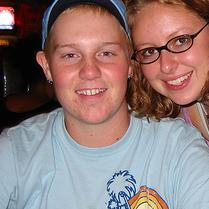
\includegraphics[width=3cm]{cap4/frontal22_1}} 
 \hspace{5mm}
 \subfloat {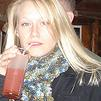
\includegraphics[width=3cm]{cap4/frontal22_2}}
 \hspace{5mm}
 \subfloat {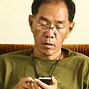
\includegraphics[width=3cm]{cap4/frontal22_3}}
 \vspace{5mm}
 
  \resizebox{.2\textwidth}{!}{%
 \begin{tabular}{|c | c|}
 \hline
 146 & 155 \\ \hline
 0 & 500 \\ 
 \hline
\end{tabular}%
}
\hspace{5mm}
\resizebox{.2\textwidth}{!}{%
\begin{tabular}{|c | c|}
 \hline
 2 & 299 \\ \hline
 0 & 500 \\ 
 \hline
\end{tabular}%
}
\hspace{5mm}
\resizebox{.2\textwidth}{!}{%
\begin{tabular}{|c | c|}
 \hline
 168 & 133 \\ \hline
 1 & 499 \\ 
 \hline
\end{tabular}%
}
\caption{Matrici di confusione per i classificatori-poselets tipo 5}
\label{table-deepnet}
 \end{figure}
 

 \section{Esempi esecuzione}
 Di seguito vediamo un esempio di esecuzione completo del software relativo al rilevamento dei bounding boxes delle persone nell'immagine.\\
 \begin{figure}[h!b]
 \centering
 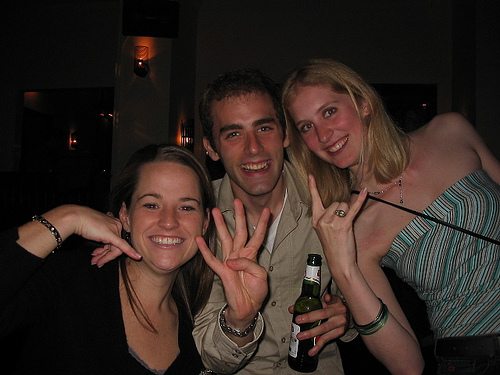
\includegraphics[scale=0.6]{cap4/test_image}
 \caption{Immagine target con tre persone}
 \label{fig:my_label}
 \end{figure}
 
\begin{lstlisting}[h!b]
 >> demo_test
R-CNN startup done
configuring person
Initializing R-CNN model (this might take a little while)
done
Extracting activations from image
Scale = 1.2
Scale = 1
Scale = 0.8
Scale = 0.6
Scale = 0.4
Scale = 0.2
Found 392 activations
Time to detect poselets in image 39.850s
Time to detect bounding boxes in image 40.882s
 \end{lstlisting}
 

 
 \begin{figure}[h]
 \centering
 \subfloat {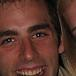
\includegraphics[scale=1]{cap4/test_act1}}
 \hspace{5mm}
 \subfloat {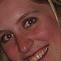
\includegraphics[scale=1]{cap4/test_act2}}
 \hspace{5mm}
 \subfloat {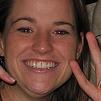
\includegraphics[scale=1]{cap4/test_act3}}

 \subfloat {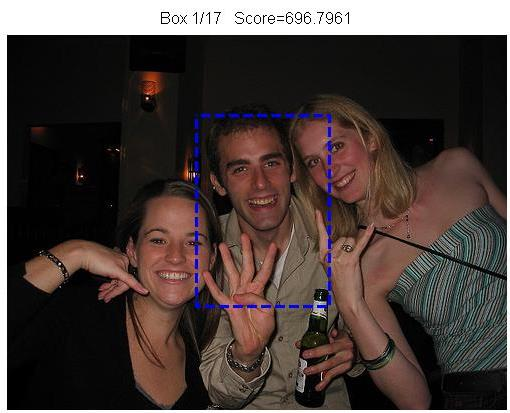
\includegraphics[scale=0.4]{cap4/test_my1}}
 \hspace{5mm}
 \subfloat {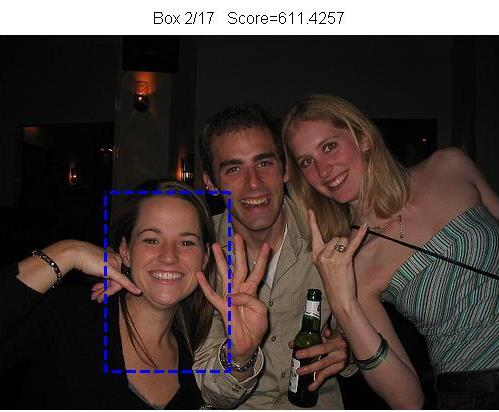
\includegraphics[scale=0.4]{cap4/test_my2}}
 \hspace{5mm}
 \subfloat {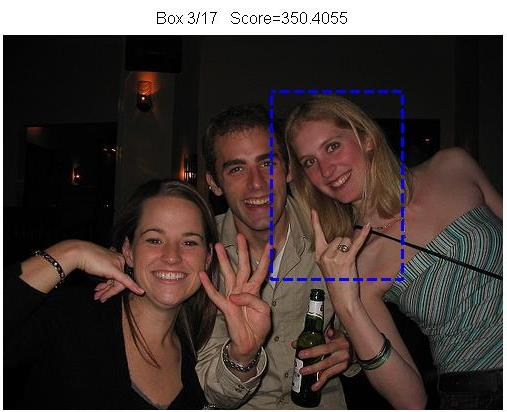
\includegraphics[scale=0.4]{cap4/test_my3}}

 \newline
 \subfloat {\includegraphics[scale=0.4]{cap4/test_my_rcnn1}}
 \hspace{5mm}
 \subfloat {\includegraphics[scale=0.4]{cap4/test_my_rcnn2}}
 
  \subfloat {\includegraphics[scale=0.4]{cap4/test_rcnn1}}
 \hspace{5mm}
 \subfloat {\includegraphics[scale=0.4]{cap4/test_rcnn2}}
 \hspace{5mm}
 \subfloat {\includegraphics[scale=0.4]{cap4/test_rcnn3}}
\caption{\textbf{Prima riga:} 3 attivazioni-poselet \textbf{Seconda riga:} Primi 3 bounding boxes rilevati dall'approccio. \newline \textbf{Terza riga} Classificazione bounding boxes rilevati da parte di R-CNN\newline
 \textbf{Quarta riga}: Selective Search Candidates + Classificazione mediante R-CNN }
 \end{figure}
 
 Vediamo dalle immagini come R-CNN non riesca a trovare il bounding box che contenga la sola persona al centro. Questo è dovuto a due motivi: il primo è che il classificatore SVM è addestrato per individuare l'intera persona e non parti di esso, il secondo è dovuto all'algoritmo utilizzato per estrapolare le regioni all'interno dell'immagine il quale non sempre funziona a dovere.\\
 
  \begin{figure}[h]
 \centering
 \subfloat {\includegraphics[scale=1]{cap4/test2_act1}}
 \hspace{5mm}
 \subfloat {\includegraphics[scale=1]{cap4/test2_act2}}
 \hspace{5mm}
 \subfloat {\includegraphics[scale=1]{cap4/test2_act3}}

 \newline
 \subfloat {\includegraphics[scale=0.4]{cap4/test2_my1}}
 \hspace{5mm}
 \subfloat {\includegraphics[scale=0.4]{cap4/test2_my2}}
 \hspace{5mm}
 \subfloat {\includegraphics[scale=0.4]{cap4/test2_my3}}

 \newline
 \subfloat {\includegraphics[scale=0.4]{cap4/test2_my_rcnn1}}
 \hspace{5mm}
 \subfloat {\includegraphics[scale=0.4]{cap4/test2_my_rcnn2}}
 \hspace{5mm}
 \subfloat {\includegraphics[scale=0.4]{cap4/test2_my_rcnn3}}
 
 \subfloat {\includegraphics[scale=0.4]{cap4/test2_rcnn1}}
 \hspace{5mm}
 \subfloat {\includegraphics[scale=0.4]{cap4/test2_rcnn2}}
 \hspace{5mm}
 \subfloat {\includegraphics[scale=0.4]{cap4/test2_rcnn3}}
 \caption{\textbf{Prima riga:} 3 attivazioni-poselet \textbf{Seconda riga:} Primi 3 bounding boxes rilevati dall'approccio. \newline \textbf{Terza riga} Classificazione bounding boxes rilevati da parte di R-CNN\newline
 \textbf{Quarta riga}: Selective Search Candidates + Classificazione mediante R-CNN }
 \end{figure}
 
 Nella seconda esecuzione, notiamo che i primi due bounding boxes sono gli stessi sia per l'approccio implementato (score bounding boxes dato dalla somma degli score delle activations all'interno), sia dopo la classificazione di R-CNN. Vediamo come R-CNN col semplice Selective Search Candidates non dia risultati esatti.
\begin{thebibliography}{30}

\bibitem{rcnn} R. Girshick, J. Donahue, T. Darrell, and J. Malik, Rich feature hierarchies for accurate object detection and semantic segmentation. arXiv preprint:1311.2524\\


\bibitem{poselets} L. Bourdev and J. Malik. Poselets: Body part detectors trained using 3D human pose annotations. In \textit{International Conference on Computer Vision (ICCV)}, 2009.

\bibitem{poselets-image} Poselets for the Person category
\url{https://www.eecs.berkeley.edu/Research/Projects/CS/vision/shape/poselets/poselets_person.html}

\bibitem{poselet-code} Poselet and Their Applications in High-Level Computer Vision
\url{https://www.eecs.berkeley.edu/Research/Projects/CS/vision/shape/poselets/}

\bibitem{coco} Microsoft COCO Dataset
\url{http://mscoco.org/dataset/#download}

\bibitem{pascal2011} Visual Object Classes Challenge 2011 (VOC2011)
\url{http://host.robots.ox.ac.uk/pascal/VOC/voc2011/index.html#data}

\bibitem{pascal-keypoints}Lubomir Bourdev and Subhransu Maji and Jitendra Malik, Detection, Attribute Classification and Action Recognition of People using Poselets (in submission), IEEE Transactions on Pattern Analysis and Machine Intelligence

\bibitem{r-cnn}Ross Girshick Jeff Donahue Trevor Darrell Jitendra Malik, Rich feature hierarchies for accurate object detection and semantic segmentation,\textit{UC Berkeley}

\bibitem{matlab} Matlab
\url{http://it.mathworks.com/products/matlab/}

\bibitem{theano} Theano
\url{http://deeplearning.net/software/theano/}

\bibitem{pylearn2} Pylearn2
\url{http://deeplearning.net/software/pylearn2/}

\bibitem{cuda} CUDA
\url{http://www.nvidia.it/object/cuda-parallel-computing-it.html}

\bibitem{conv-3x} 3x faster convolutions in Theano
\url{http://benanne.github.io/2014/04/03/faster-convolutions-in-theano.html}

\bibitem{caffe} Caffe
\url{http://caffe.berkeleyvision.org/}

\end{thebibliography}


\newpage
\pagestyle{plain}

%\input{tesi_tex/ringraziamenti.tex}

\end{document}
